\begin{figure*}[t!]
\centering
\begin{subfigure}[h]{\textwidth}
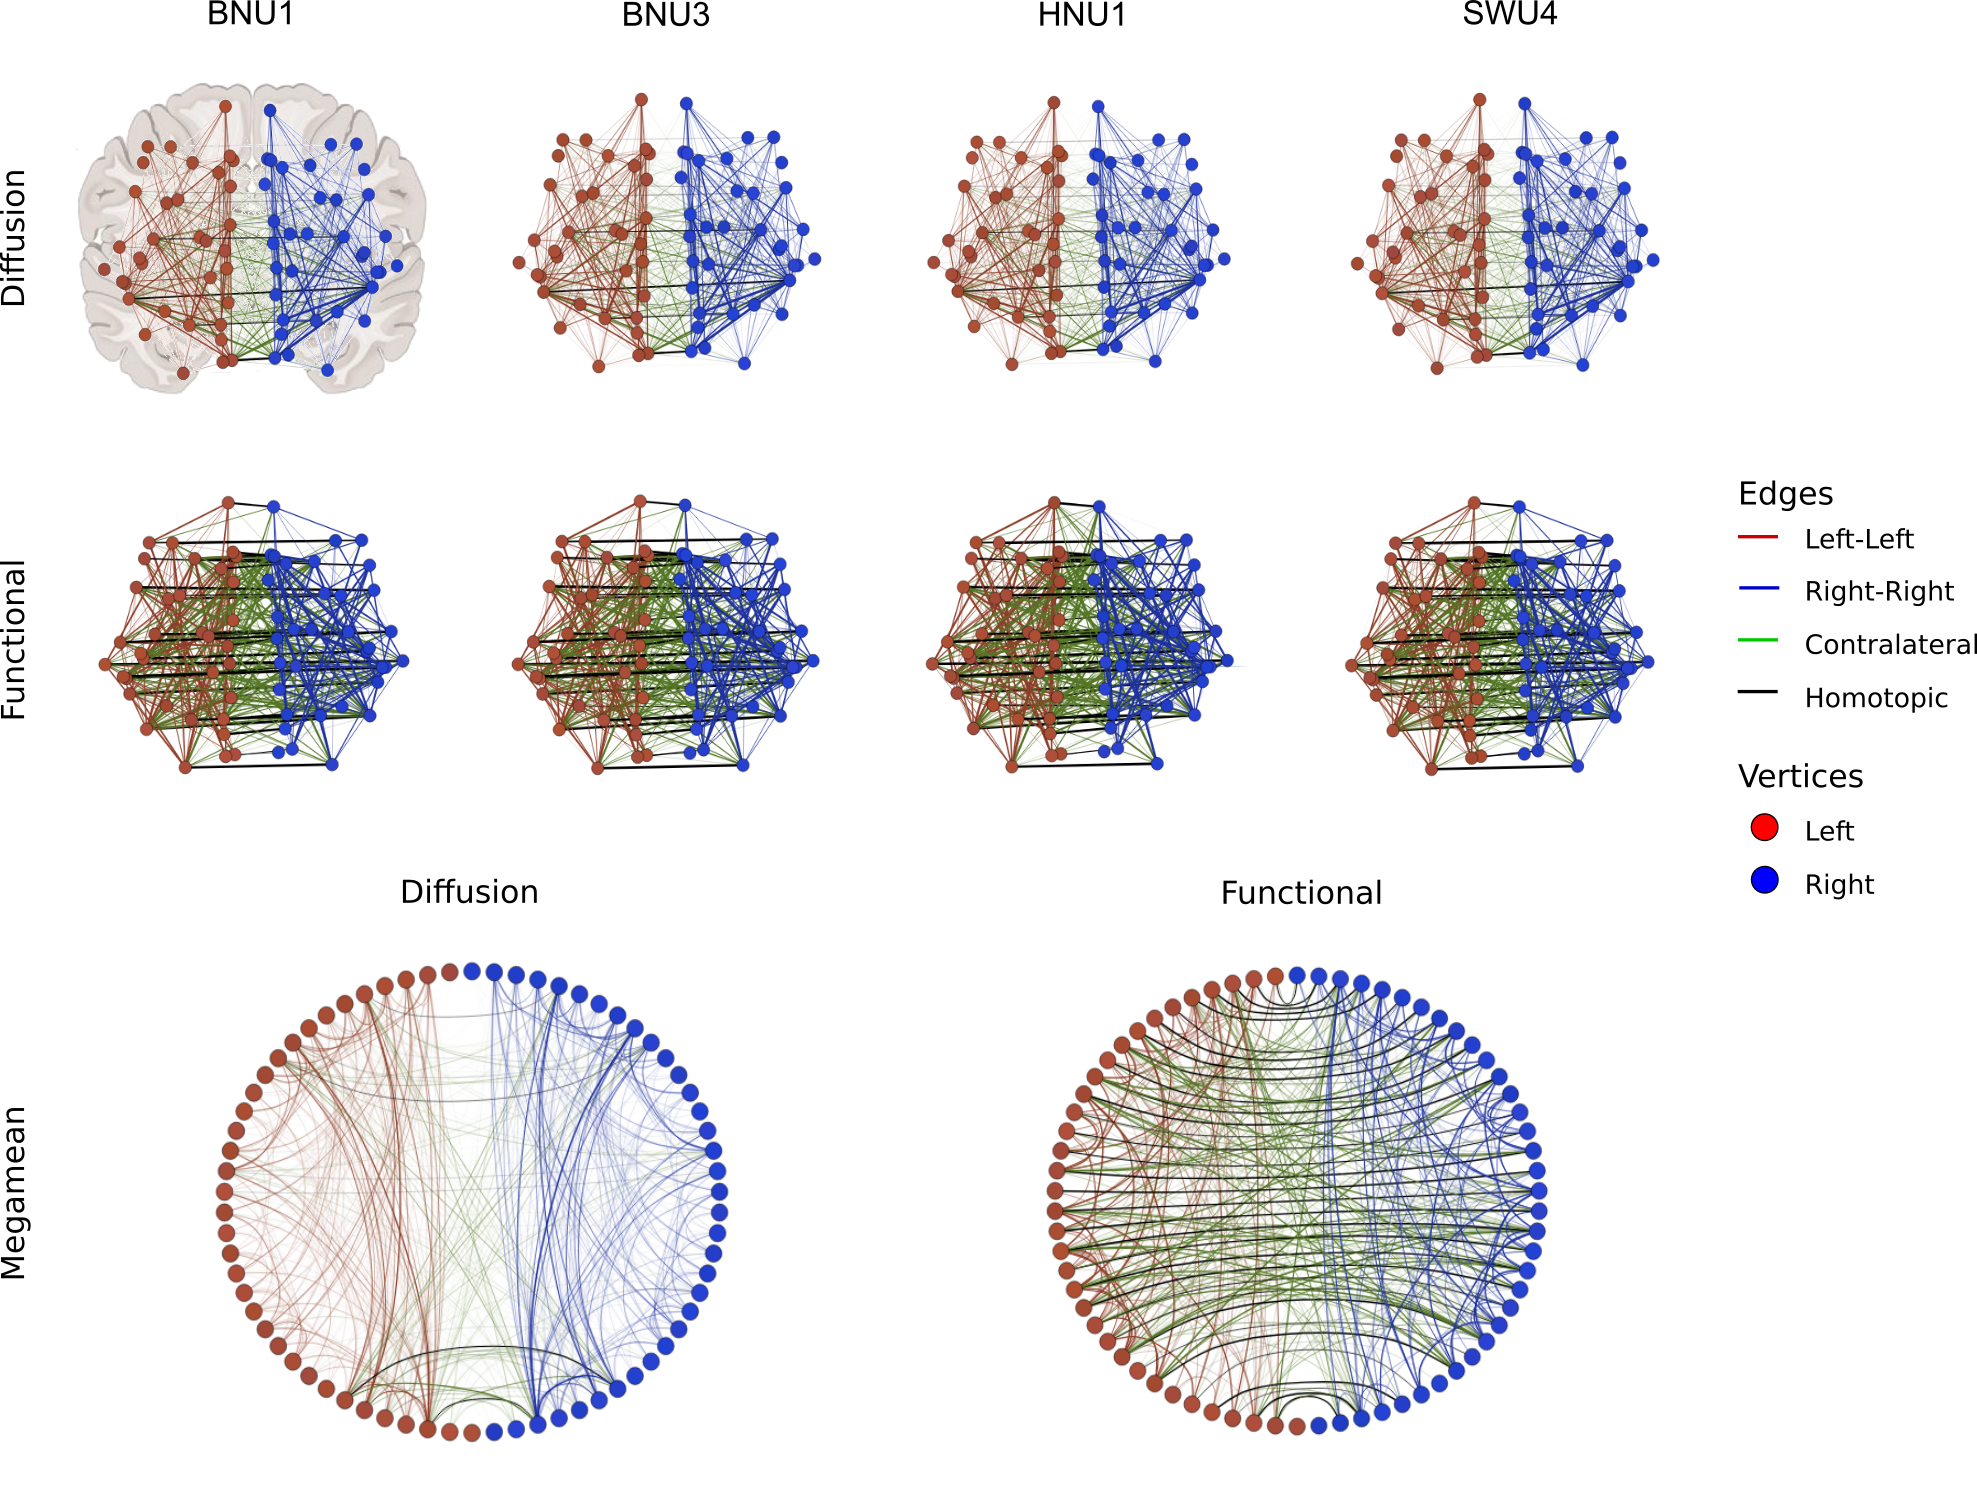
\includegraphics[width=\textwidth]{./megamean/megamean.png}
\end{subfigure}
\caption{\textbf{Multi-Study Mean Connectomes}. 
Site-specific mean connectomes (top two rows) and mega-mean (bottom row), using the Desikan parcellation, 
%Dataset-mean connectomes and a combined mean-of-mean Desikan labeled graphs 
%produced by \ndmg, 
%resulting in the largest
%known mean connectome to-date, 
using all the data for which we have both functional and diffusion studies ($>900$ scans of each), with edges and vertices colored depending on hemisphere.
%Bilateral edges connecting the same regions in opposite hemispheres are shown in black. 
In the top 2 rows, graphs are shown with vertex position determined by the coronally-projected center of mass for each region in the Desikan parcellation.  The bottom shows radial plots organized by hemisphere.
Same-modality connectomes appear qualitatively similar to one another across sites, but some differences across modalities are apparent.  For example, 
homotopic and contralateral connections both seem stronger in functional than diffusion mean connectomes, both within site and after pooling all sites.
%, ipsi-lateral connectivity in the diffusion connectomes is consistently more dense than contra-lateral
%connectivity in the functional connectomes. 
%Likewise, homotopic connectivity in the functional connectomes appears more dense than heterotopic connectivity in the diffusion connectomes.
}
\label{fig:mean}
\end{figure*}